\documentclass[10pt]{beamer}

\usepackage{amsfonts}
\usepackage{subfiles}
\usepackage[T2A]{fontenc}
\usepackage[utf8]{inputenc}
\usepackage[russian]{babel}

\usepackage{amsmath, amsfonts, amssymb, amsthm, mathtools, mathrsfs}
\usepackage{wasysym, dsfont}
\usepackage{graphicx}
\usepackage{float}
\usepackage{wrapfig}
\usepackage{subcaption}
\usepackage{multirow}
\usepackage{caption}
\usepackage{subcaption}

\usepackage{multicol}
\DeclareMathOperator*{\argmax}{\arg\!\max}
\DeclareMathOperator*{\argmin}{\arg\!\min}

\mode<presentation>
{
	\usetheme{boxes}
	\beamertemplatenavigationsymbolsempty
	
	\setbeamertemplate{footline}[page number]
	\setbeamersize{text margin left=1.5em, text margin right=2.0em}
}
\newcommand\blfootnote[1]{%
	\begingroup
	\renewcommand\thefootnote{}\footnote{#1}%
	\addtocounter{footnote}{-1}%
	\endgroup
}
\newcommand\FontUP{\fontsize{12}{12}\selectfont}


\title[]{Improving algorithmic alignment with autoregressive memory}

\author{Nikita Okhotnikov}
\date{2024}

\begin{document}

\begin{frame}
  \titlepage

\end{frame}

\begin{frame}{Introduction}
	\begin{itemize}
		\item \dots
	\end{itemize}
\end{frame}

\begin{frame}{Algorithmic alignment}
	\begin{block}{Definition 1}
		$\varepsilon >0 $ -- error parameter, $\delta\in (0,1)$ -- error probability. 
		$\{x_i, y_i\}_{i=1}^M$ -- i.i.d from $\mathcal{D}$ and $y_i = g(x_i)$ for some function $g$. Let
		$f = \mathcal{A}(\{x_i, y_i\}_{i=1}^M)$ be the function generated by a learning algorithm $\mathcal{A}$.
		Then $g$ is $(M, \varepsilon, \delta)$-\textit{learnable} with $\mathcal{A}$ if 
		$$\mathbb{P}_{x\sim \mathcal{D}}\left[\|f(x)-g(x)\|\leq \varepsilon\right] \geq 1-\delta$$ 
	\end{block}
	\begin{block}{Definition 2}
		\textit{Sample complexity} $\mathcal{C}_\mathcal{A}(g, \varepsilon, \delta)$ is the minimum $M$ so that $g$
		is $(M, \varepsilon, \delta)$-learnable with $\mathcal{A}$.
	\end{block}
	\begin{block}{Definition 3}
		Let $g$ be a reasoning function, $\mathcal{N}$ -- neural network with $n$ modules $\mathcal{N}_i$. 
		Module functions $f_1, \dots, f_n$ generate $g$ for $\mathcal{N}$ if, by replacing $\mathcal{N}_i$ with $f_i$, the network $\mathcal{N}$ simulates $g$. 
		Then $\mathcal{N}$ $(M, \varepsilon, \delta)$-\textit{algorithmically aligns} with $g$ if $f_1, \dots, f_n$ generate $g$ and 
		there are learning algorithms $\mathcal{A}_i$ for the $\mathcal{N}_i$ such that $n\cdot\max_i C_{\mathcal{A}_i}(f_i, \varepsilon, \delta)\leq M$.	
	\end{block}
\end{frame}

\begin{frame}{Algorithmic alignment impoves sample complexity}
	\begin{block}{Theorem 1 (Keyulu Xu, et. al. 2020)}
		$\mathcal{A}$ -- an overparameterized and randomly initialized 2-layer MLP trained with GD for a sufficient number of iterations.
		Suppose $g:~\mathbb{R}^d\to \mathbb{R}^m$ with components $g(x)^{(i)} = \sum_j \alpha_j^{(i)} \left(\beta_j^{(i)\top}x\right)^{p_j^{(i)}}$, where
		$\beta_j^{(i)}\in \mathbb{R}^d,~\alpha\in\mathbb{R}$ and $p_j^{(i)} = 1$ or $p_j^{(i)} = 2l,~(l\in \mathbb{N})$. 
		Then the sample complexity $\mathcal{C}(g, \varepsilon, \delta)$ is 
		\vspace{-0.4cm}
		\[\mathcal{C}_\mathcal{A}(g, \varepsilon, \delta) = O\left( \frac{\max_i\sum_{j=1}^{K} p_j^{(i)}|\alpha_j^{(i)}|\cdot\|\beta_j^{(i)}\|_2^{p_j^{(i)}} + \log (m / \delta)}{(\varepsilon / m)^2} \right)\]
	\end{block}

	\begin{block}{Theorem 2 (Keyulu Xu, et. al. 2020)}
		For some $\varepsilon, \delta$ suppose $\{S_i, y_i\}_{i=1}^M\sim \mathcal{D}, ~|S_i|< N,~ y_i = g(S_i)$ for some $g$. 
		Suppose $\mathcal{N}_1\dots \mathcal{N}_n$ are sequential MLP modules of $\mathcal{N}$. Suppose $\mathcal{N}$ and $g$ $(M, \varepsilon, \delta)$-algorithmically align via $f_1\dots f_n$.	
		Then $g$ is $(M, O(\varepsilon), O(\delta))$-learnable by $\mathcal{N}$.
	\end{block}

	\begin{block}{Corollary 1}
		Suppose universe $S$ has $n$ objects $x_1\dots x_n$ and $g(S) = \sum_{i,j} (x_i - x_j)^2$. Then the sample complexity 
		of MLP is $O(n^2)$ times larger than that of GNN.
	\end{block}
\end{frame}


\begin{frame}{Neural algorithmic reasoning, processor network}
	\begin{center}
		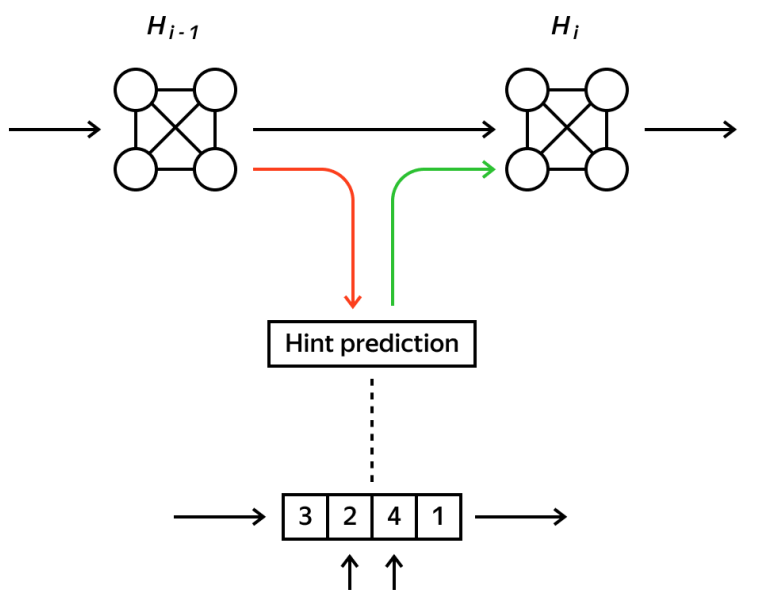
\includegraphics[scale=0.3]{../pictures/processor with hints.png}
	\end{center}
	\begin{itemize}
		\item Trained to follow trajectory of classical algorithm
		\item Aligns poorly with multiple algorithms at once
		\item Needs implicit hints on each step to enforce trajectory following
	\end{itemize}
\end{frame}


\begin{frame}{Processor network with autoregressive memory}
	\begin{center}
		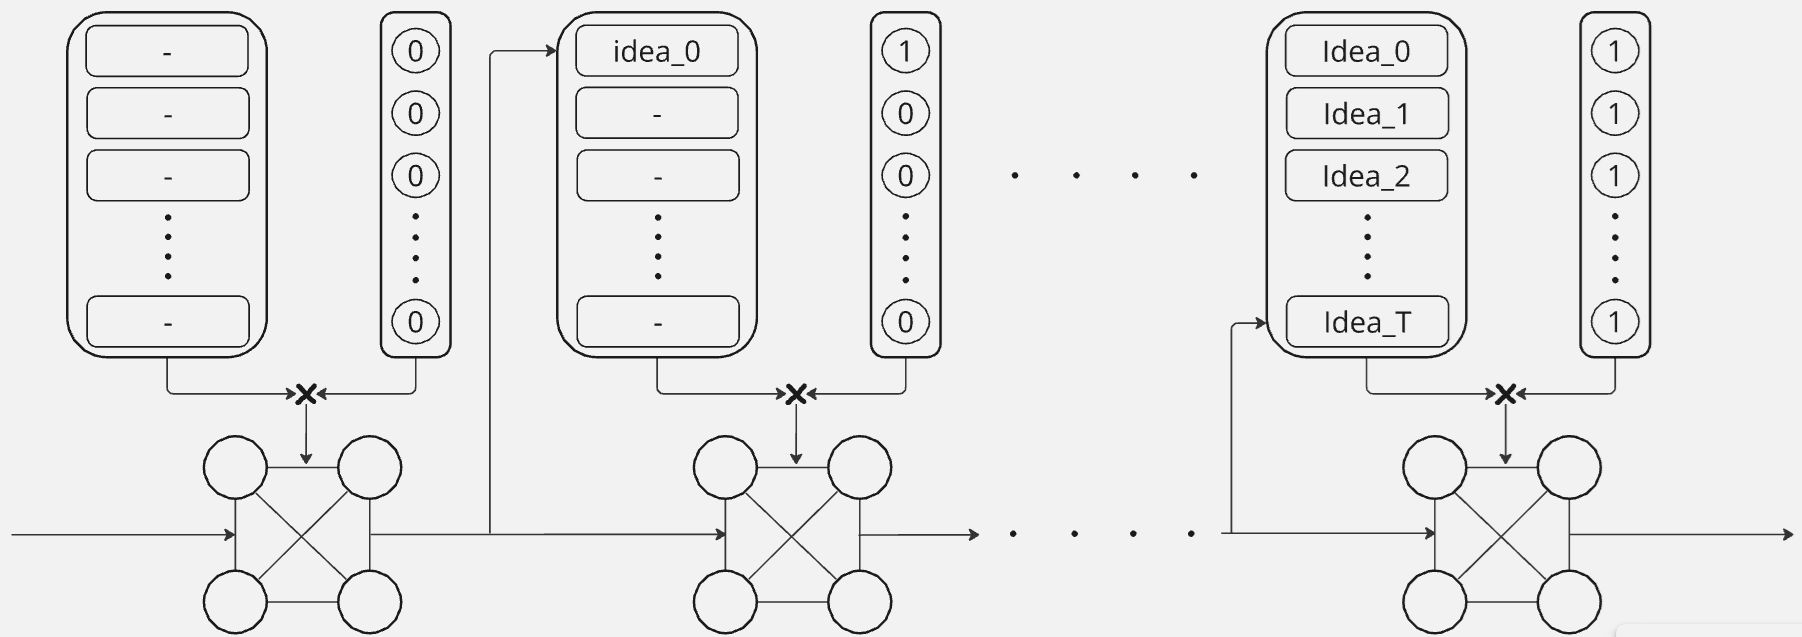
\includegraphics[scale=0.25]{../pictures/extra-ARM-GNN.png}
	\end{center}
	\begin{equation*}
		L = - \sum_{X\in \mathcal{X}}\sum\limits_{X_a \in \mathcal{X}_X}\log\frac{  \exp{\left(  \sum\limits_{t=1}^{T} \phi\left(M_t^X, M_t^{X_a}\right)  \right)}  }{  \exp{\left(  \sum_{t=1}^{T} \phi\left(M_t^X, M_t^{X_a}\right)  \right)} + \sum\limits_{\overline{X_a}\in \overline{\mathcal{X}_X}}\exp\left(\sum\limits_{t=1}^{T}\phi\left(M_t^X, M_t^{\overline{X_a}}\right)\right)  }
	\end{equation*}
		$\mathcal{X}$ -- set of inputs, $M_t^X\in \mathbb{R}^k$ -- the <<idea>> generated on step $t$ for input $X$, $\mathcal{X}_X$ -- set of inputs similar to $X$, $\overline{\mathcal{X}_X}$ -- set of inputs dissimilar to $X$
\end{frame}

\begin{frame}{Processor network with autoregressive memory}
	\begin{itemize}
		\item Mimics the step-by-step behaviour of classical algorithms not the exact trajectories
		\item Much less constraint compared to usual hint-prediction approach
		\item Does not require explicit hints
		\item Force processor to extract similar features (<<ideas>>) for similar algorithms at each step that might help with multi-algorithm learning
	\end{itemize}
\end{frame}




\end{document}